\documentclass[12pt]{article}
\linespread{1}

% margins
\setlength{\textwidth}{6.5in}
\setlength{\textheight}{8.75in}
\setlength{\oddsidemargin}{-0.1in}
\setlength{\topmargin}{-0.1in}
\setlength{\baselineskip}{10pt}

% load packages
\usepackage{amsmath}
\usepackage{amsfonts}
\usepackage{lscape}
\usepackage[round]{natbib}
\usepackage{graphicx}
\graphicspath{{figures/}}
\usepackage{amssymb}
\usepackage{color}
\usepackage{hyperref}
\usepackage{booktabs}
\usepackage{verbatim}
\usepackage{longtable}

% style setup
\bibliographystyle{plainnat}
\pagestyle{empty}
\setlength\parindent{0pt}
\setlength{\parskip}{\baselineskip}

% new commands
\newcommand{\indist}{\overset{d}{\rightarrow}}
\newcommand{\inprob}{\overset{P}{\rightarrow}}
\newcommand{\tabby}{\hspace{10pt}}
\newcommand{\ones}{{\bf 1}}
\newcommand{\tp}{\intercal}
\newcommand{\iprod}[2]{\langle #1 , #2 \rangle}

\newcommand{\note}[1]{\textcolor{red}{#1}}

% header
\title{HOSEA Aim I -- Report}
\author{Simon Fontaine}
\date{\today}

\begin{document}

\maketitle




\section{Current status}

\subsection{Comparison}

\subsubsection{ANY}

\begin{figure}[ht]
\includegraphics[width=1.0\linewidth]{comparison/ANY_imputed.pdf}
\end{figure}

\begin{figure}[ht]
\includegraphics[width=1.0\linewidth]{comparison/ANY_complete.pdf}
\end{figure}

\begin{figure}[ht]
\includegraphics[width=1.0\linewidth]{comparison/ANY_incomplete.pdf}
\caption{This should read ``incomplete''...}
\end{figure}

\clearpage
\newpage
\subsubsection{EAC}

\begin{figure}[ht]
\includegraphics[width=1.0\linewidth]{comparison/EAC_imputed.pdf}
\end{figure}

\begin{figure}[ht]
\includegraphics[width=1.0\linewidth]{comparison/EAC_complete.pdf}
\end{figure}

\begin{figure}[ht]
\includegraphics[width=1.0\linewidth]{comparison/EAC_incomplete.pdf}
\caption{This should read ``incomplete''...}
\end{figure}

\clearpage
\newpage
\subsubsection{EGJAC}

\begin{figure}[ht]
\includegraphics[width=1.0\linewidth]{comparison/EGJAC_imputed.pdf}
\end{figure}

\begin{figure}[ht]
\includegraphics[width=1.0\linewidth]{comparison/EGJAC_complete.pdf}
\end{figure}

\begin{figure}[ht]
\includegraphics[width=1.0\linewidth]{comparison/EGJAC_incomplete.pdf}
\caption{This should read ``incomplete''...}
\end{figure}


\newpage
\clearpage
\subsection{Calibration}


\begin{figure}[ht]
\includegraphics[width=1.0\linewidth]{calibration/ANY_imputed.pdf}
\end{figure}
\begin{figure}[ht]
\includegraphics[width=1.0\linewidth]{calibration/EAC_imputed.pdf}
\end{figure}
\begin{figure}[ht]
\includegraphics[width=1.0\linewidth]{calibration/EGJAC_imputed.pdf}
\end{figure}



\newpage
\clearpage
\subsection{Threshold}

% latex table generated in R 4.2.0 by xtable 1.8-4 package
% Mon Sep 12 11:35:51 2022
\begin{table}[t]
\centering
\tiny
\begin{tabular}{lccc}
  \toprule
  \multicolumn{4}{l}{\textbf{ANY}} \\\addlinespace
Threshold & TPR & PPV & DetPrevalence \\ 
  \midrule
0 & 100.00 & 0.11 & 100.00 \\ 
  5 & 99.54 & 0.13 & 82.38 \\ 
  10 & 99.40 & 0.14 & 78.88 \\ 
  15 & 99.09 & 0.15 & 75.76 \\ 
  20 & 98.60 & 0.15 & 72.73 \\ 
   \addlinespace
25 & 97.68 & 0.16 & 69.71 \\ 
  30 & 97.16 & 0.16 & 66.67 \\ 
  35 & 96.10 & 0.17 & 63.70 \\ 
  40 & 95.19 & 0.17 & 60.83 \\ 
  45 & 94.24 & 0.18 & 58.08 \\ 
   \addlinespace
50 & 93.22 & 0.19 & 55.47 \\ 
  55 & 92.17 & 0.19 & 52.98 \\ 
  60 & 91.12 & 0.20 & 50.60 \\ 
  65 & 89.68 & 0.21 & 48.36 \\ 
  70 & 88.24 & 0.21 & 46.22 \\ 
   \addlinespace
75 & 86.73 & 0.22 & 44.21 \\ 
  80 & 85.32 & 0.22 & 42.32 \\ 
  85 & 84.23 & 0.23 & 40.53 \\ 
  90 & 82.94 & 0.24 & 38.87 \\ 
  95 & 81.64 & 0.24 & 37.30 \\ 
   \addlinespace
100 & 80.65 & 0.25 & 35.81 \\ 
  105 & 79.39 & 0.26 & 34.39 \\ 
  110 & 77.98 & 0.26 & 33.06 \\ 
  115 & 76.65 & 0.27 & 31.78 \\ 
  120 & 75.42 & 0.27 & 30.57 \\ 
   \addlinespace
125 & 73.98 & 0.28 & 29.41 \\ 
  130 & 72.75 & 0.29 & 28.30 \\ 
  135 & 71.52 & 0.29 & 27.24 \\ 
  140 & 70.19 & 0.30 & 26.23 \\ 
  145 & 68.71 & 0.30 & 25.24 \\ 
   \addlinespace
150 & 67.10 & 0.31 & 24.30 \\ 
  155 & 65.77 & 0.31 & 23.39 \\ 
  160 & 64.64 & 0.32 & 22.51 \\ 
  165 & 63.38 & 0.32 & 21.66 \\ 
  170 & 62.08 & 0.33 & 20.85 \\ 
   \addlinespace
175 & 61.17 & 0.34 & 20.07 \\ 
  180 & 59.59 & 0.34 & 19.33 \\ 
  185 & 58.39 & 0.35 & 18.61 \\ 
  190 & 57.09 & 0.35 & 17.93 \\ 
  195 & 56.04 & 0.36 & 17.27 \\ 
   \addlinespace
200 & 54.95 & 0.37 & 16.64 \\ 
  220 & 50.49 & 0.39 & 14.38 \\ 
  240 & 46.52 & 0.41 & 12.50 \\ 
  260 & 42.84 & 0.44 & 10.92 \\ 
  280 & 39.54 & 0.46 & 9.56 \\ 
   \addlinespace
300 & 37.18 & 0.49 & 8.40 \\ 
  320 & 34.02 & 0.51 & 7.41 \\ 
  340 & 31.07 & 0.53 & 6.56 \\ 
  360 & 29.14 & 0.56 & 5.81 \\ 
  380 & 26.83 & 0.58 & 5.16 \\ 
   \addlinespace
400 & 24.72 & 0.60 & 4.59 \\ 
  420 & 23.24 & 0.63 & 4.09 \\ 
  440 & 21.38 & 0.65 & 3.65 \\ 
  460 & 19.73 & 0.67 & 3.26 \\ 
  480 & 18.64 & 0.71 & 2.92 \\ 
   \addlinespace
500 & 17.38 & 0.74 & 2.62 \\ 
  550 & 14.54 & 0.81 & 2.00 \\ 
  600 & 12.46 & 0.90 & 1.53 \\ 
  650 & 10.29 & 0.96 & 1.19 \\ 
  700 & 8.25 & 0.98 & 0.93 \\ 
   \addlinespace
750 & 7.16 & 1.08 & 0.73 \\ 
  800 & 5.76 & 1.09 & 0.58 \\ 
  850 & 4.88 & 1.16 & 0.47 \\ 
  900 & 4.39 & 1.30 & 0.37 \\ 
  950 & 3.79 & 1.38 & 0.31 \\ 
   \addlinespace
1000 & 3.41 & 1.52 & 0.25 \\ 
   \bottomrule
\end{tabular}
\end{table}


\input{tables/calibration/thresholds_EAC_imputed.tex}

% latex table generated in R 4.2.0 by xtable 1.8-4 package
% Mon Sep 12 11:42:50 2022
\begin{table}[ht]
\centering
\begin{tabular}{lccc}
  \toprule
Threshold & TPR & PPV & DetPrevalence \\ 
  \midrule
0 & 100.00 & 0.03 & 100.00 \\ 
  5 & 98.58 & 0.04 & 76.82 \\ 
  10 & 96.11 & 0.04 & 65.06 \\ 
  15 & 89.25 & 0.05 & 53.93 \\ 
  20 & 83.68 & 0.06 & 44.85 \\ 
   \addlinespace
25 & 77.72 & 0.06 & 37.42 \\ 
  30 & 70.85 & 0.07 & 31.35 \\ 
  35 & 64.64 & 0.07 & 26.37 \\ 
  40 & 58.55 & 0.08 & 22.29 \\ 
  45 & 53.89 & 0.09 & 18.91 \\ 
   \addlinespace
50 & 48.32 & 0.09 & 16.12 \\ 
  55 & 43.26 & 0.09 & 13.78 \\ 
  60 & 38.99 & 0.10 & 11.84 \\ 
  65 & 34.97 & 0.10 & 10.23 \\ 
  70 & 30.83 & 0.10 & 8.87 \\ 
   \addlinespace
75 & 27.85 & 0.11 & 7.71 \\ 
  80 & 25.26 & 0.11 & 6.73 \\ 
  85 & 22.54 & 0.11 & 5.90 \\ 
  90 & 19.56 & 0.11 & 5.19 \\ 
  95 & 18.01 & 0.12 & 4.58 \\ 
   \addlinespace
100 & 16.84 & 0.12 & 4.06 \\ 
  105 & 15.41 & 0.13 & 3.60 \\ 
  110 & 14.51 & 0.14 & 3.20 \\ 
  115 & 12.82 & 0.14 & 2.86 \\ 
  120 & 11.40 & 0.13 & 2.55 \\ 
   \addlinespace
125 & 10.23 & 0.13 & 2.28 \\ 
  130 & 8.94 & 0.13 & 2.05 \\ 
  135 & 8.16 & 0.13 & 1.84 \\ 
  140 & 7.38 & 0.13 & 1.66 \\ 
  145 & 6.87 & 0.14 & 1.50 \\ 
   \addlinespace
150 & 6.35 & 0.14 & 1.36 \\ 
  155 & 5.96 & 0.15 & 1.23 \\ 
  160 & 5.83 & 0.16 & 1.12 \\ 
  165 & 5.05 & 0.15 & 1.02 \\ 
  170 & 4.79 & 0.16 & 0.92 \\ 
   \addlinespace
175 & 4.27 & 0.15 & 0.84 \\ 
  180 & 4.27 & 0.17 & 0.77 \\ 
  185 & 4.15 & 0.18 & 0.70 \\ 
  190 & 4.02 & 0.19 & 0.64 \\ 
  195 & 3.63 & 0.19 & 0.59 \\ 
   \addlinespace
200 & 3.37 & 0.19 & 0.54 \\ 
  220 & 2.46 & 0.19 & 0.39 \\ 
  240 & 2.07 & 0.22 & 0.28 \\ 
  260 & 1.55 & 0.22 & 0.21 \\ 
  280 & 1.17 & 0.22 & 0.16 \\ 
   \addlinespace
300 & 0.78 & 0.20 & 0.12 \\ 
  320 & 0.78 & 0.26 & 0.09 \\ 
  340 & 0.39 & 0.17 & 0.07 \\ 
  360 & 0.39 & 0.21 & 0.05 \\ 
  380 & 0.39 & 0.27 & 0.04 \\ 
   \addlinespace
400 & 0.39 & 0.34 & 0.03 \\ 
  420 & 0.13 & 0.14 & 0.03 \\ 
  440 & 0.13 & 0.18 & 0.02 \\ 
  460 & 0.13 & 0.22 & 0.02 \\ 
  480 & 0.13 & 0.28 & 0.01 \\ 
   \addlinespace
500 & 0.13 & 0.34 & 0.01 \\ 
  550 & 0.13 & 0.53 & 0.01 \\ 
  600 & 0.00 & 0.00 & 0.00 \\ 
  650 & 0.00 & 0.00 & 0.00 \\ 
  700 & 0.00 & 0.00 & 0.00 \\ 
   \addlinespace
750 & 0.00 & 0.00 & 0.00 \\ 
  800 & 0.00 & 0.00 & 0.00 \\ 
  850 & 0.00 & 0.00 & 0.00 \\ 
  900 & 0.00 & 0.00 & 0.00 \\ 
  950 & 0.00 & 0.00 & 0.00 \\ 
   \addlinespace
1000 & 0.00 & 0.00 & 0.00 \\ 
   \bottomrule
\end{tabular}
\end{table}




\newpage
\clearpage
\subsection{Identity}


\begin{figure}[ht]
\includegraphics[width=1.0\linewidth]{identity/ANY_age.pdf}
\end{figure}
\begin{figure}[ht]
\includegraphics[width=1.0\linewidth]{identity/ANY_sex.pdf}
\end{figure}
\begin{figure}[ht]
\includegraphics[width=1.0\linewidth]{identity/ANY_race.pdf}
\end{figure}



\newpage
\clearpage
\subsection{Representative samples}


\begin{figure}[ht]
\includegraphics[width=1.0\linewidth]{comparison/ANY_imputed_representative.pdf}
\end{figure}
\begin{figure}[ht]
\includegraphics[width=1.0\linewidth]{comparison/ANY_complete_representative.pdf}
\end{figure}
\begin{figure}[ht]
\includegraphics[width=1.0\linewidth]{comparison/ANY_incomplete_representative.pdf}
\caption{This should read ``incomplete''...}
\end{figure}

\newpage
\clearpage
\subsection{Variable importance}

A few observations:
\begin{itemize}
\item Age, gender, race, smoking, GERD all among the top 8 most important in terms of SHAP
\item BMI/weight much farther
\item HIV is now one of the most important
\item Important labs: WBC, NA
\item EAC: mostly similar to ANY (not surprising because of large prevalance)
\item EGJAC: Age, race, smoking, gender, GERD are all less important
\end{itemize}


\begin{figure}[ht]
\includegraphics[width=1.0\linewidth]{variable_importance/shap_cat.pdf}
\end{figure}

\begin{figure}[ht]
\includegraphics[width=1.0\linewidth]{variable_importance/shap_group.pdf}
\end{figure}


\newpage
\clearpage

\section*{Previous update}


\begin{itemize}
\item I am currently investigating the difference in performance between the update of EGJAC lab results. 
In particular, there remained a few issues:
\begin{itemize}
	\item Why is there such a difference in the EAC model? For this outcome, only a few control 
	(the EGJAC cases) changed slightly, so I do not expect significant changes
	\item Why is there such a difference between complete data (wrt to HUNT/Kunzmann) and general data? 
	Why are we doing so much worse for complete data? 
	\item Why is there a difference in the HUNT and Kunzmann results? These should not change since the data is exactly the same.
	\item Why is the performance so much worse for older patients? 
\end{itemize}
\item Findings:
\begin{itemize}
	\item Tuning: I had to tweak tuning parameters because I saw some overfitting for EGJAC; I did a few tests and this doesn't seem to be the issue
	\item Feature distribution: labs are mostly the same, differences are minor and cannot account for the various differences
	\item I verified that the test set were identical
	\item I get fewer ``complete cases'' now (407K patients, 1192 cases; 363K, 845 cases). No idea why yet. 
	This surely explains the difference in HUNT/Kunzmann scores, but should still be understood. 
	\item I can almost reproduce the past results by using [4-0] data instead of [5-1] data. There remains some small gaps, but that could be from
	the imputation, small changes in processing, etc.
	\item In terms of ``complete data'', we are now much closer: 394267 patients 1173 and cases. There remains a small gap, but that might just be small changes in processing. 
	Indeed, I used the lates processing for [4-0], while an earlier version was used.
	\item Remains to understand the shift in EAC and complete data.
\end{itemize}
\end{itemize}



I compared a few iterations:
\begin{itemize}
\item Original: the model currently in the package
\item Post EGJAC: the new model with update EGJAC
\item Pre EGJAC: Everything kept the same except for the EGJAC
\end{itemize}
I compared a few datasets:
\begin{itemize}
\item Post EGJAC: the latest dataset
\item Pre EGJAC: same, but without updated EGJAC
\item Shifted: using the post\_egjac processing, but to [4-0] data instead of [5-1]
\item c\_xxxxxx: a few processing iterations from the past
\end{itemize}


\begin{table}[ht]
\centering
\begin{tabular}{rlllll}
\toprule
& data & model & ANY & EAC & EGJAC \\
\midrule

\multicolumn{6}{c}{MICE} \\
  6 & post\_egjac & post\_egjac & \textbf{0.800} [0.793,0.807] & \textbf{0.802} [0.794,0.811] & \textbf{0.769} [0.755,0.783] \\ \addlinespace

\multicolumn{6}{c}{SRS} \\
  4 & post\_egjac & original & 0.737 [0.729,0.745] & 0.742 [0.733,0.751] & 0.646 [0.628,0.664] \\ 
  5 & post\_egjac & pre\_egjac & 0.749 [0.742,0.756] & 0.763 [0.754,0.771] & 0.593 [0.574,0.612] \\ 
  6 & post\_egjac & post\_egjac & \textbf{0.769} [0.762,0.776] & \textbf{0.771} [0.763,0.78] & \textbf{0.741} [0.725,0.756] \\ \addlinespace
1 & pre\_egjac & original & 0.797 [0.789,0.805] & 0.763 [0.754,0.773] & 0.909 [0.895,0.922] \\ 
  2 & pre\_egjac & pre\_egjac & \textbf{0.816} [0.809,0.824] & \textbf{0.79} [0.781,0.798] & \textbf{0.941} [0.931,0.951] \\ 
  3 & pre\_egjac & post\_egjac & 0.772 [0.765,0.779] & 0.772 [0.763,0.78] & 0.738 [0.723,0.753] \\ \addlinespace
  7 & c\_f6f1f465 & original & 0.806 [0.797,0.814] & 0.778 [0.768,0.787] & 0.905 [0.891,0.919] \\ 
  8 & c\_f6f1f465 & pre\_egjac & 0.819 [0.812,0.826] & 0.792 [0.783,0.8] & 0.941 [0.93,0.951] \\ 
  9 & c\_f6f1f465 & post\_egjac & 0.771 [0.764,0.778] & 0.772 [0.764,0.781] & 0.737 [0.722,0.753] \\ \addlinespace
  10 & c\_69cc9e5b & original & 0.806 [0.797,0.814] & 0.778 [0.768,0.787] & 0.905 [0.891,0.919] \\ 
  11 & c\_69cc9e5b & pre\_egjac & 0.819 [0.812,0.826] & 0.792 [0.783,0.8] & 0.941 [0.93,0.951] \\ 
  12 & c\_69cc9e5b & post\_egjac & 0.771 [0.764,0.778] & 0.772 [0.764,0.781] & 0.737 [0.722,0.753] \\ \addlinespace

1 & shifted & original & \textbf{0.879} [0.872,0.885] & \textbf{0.86} [0.853,0.868] & \textbf{0.955} [0.945,0.965] \\ 
  2 & shifted & pre\_egjac & 0.849 [0.842,0.855] & 0.821 [0.814,0.829] & 0.969 [0.962,0.977] \\ 
  3 & shifted & post\_egjac & 0.805 [0.798,0.812] & 0.807 [0.799,0.814] & 0.773 [0.759,0.787] \\ \addlinespace

 & (figures) & (figures)  & \textbf{0.898} [0.892,0.903] & \textbf{0.858} [0.842,0.873] & \textbf{0.949} [0.926,0.972] \\ \addlinespace
 
 & testing& post\_egjac & 0.781 & 0.763 & 0.741 \\
 & testing & pre\_egjac & 0.833 & 0.781 & 0.954 \\
 & testing& original & 0.920 & 0.870 & 0.970 \\
\bottomrule
\end{tabular}
\caption{This is for the full test set (25\% of controls and cases). Apart from a small difference in ANY, EAC and EGJAC are almost identical between the figures and ``shifted original''.
this is the only situation even in the same ballpark.}
\end{table}





\begin{table}[ht]
\centering
\begin{tabular}{rlllll}
\toprule
& data & model & ANY & EAC & EGJAC \\
\midrule
  6 & post\_egjac & original & 0.691 [0.675,0.707] & 0.68 [0.662,0.698] & 0.607 [0.571,0.644] \\ 
  7 & post\_egjac & pre\_egjac & 0.704 [0.689,0.72] & 0.727 [0.71,0.743] & 0.61 [0.573,0.647] \\ 
  8 & post\_egjac & post\_egjac & \textbf{0.714} [0.699,0.728] & \textbf{0.736} [0.72,0.753] & \textbf{0.681} [0.649,0.713] \\ 
  9 & post\_egjac & Kunzmann & 0.637 [0.62,0.654] & 0.635 [0.616,0.653] & 0.64 [0.604,0.676] \\ 
  10 & post\_egjac & HUNT & 0.597 [0.579,0.616] & 0.615 [0.594,0.636] & 0.625 [0.589,0.66] \\ \addlinespace
 1 & pre\_egjac & original & 0.811 [0.796,0.827] & 0.745 [0.727,0.763] & 0.991 [0.987,0.996] \\ 
  2 & pre\_egjac & pre\_egjac & \textbf{0.814} [0.799,0.828] & \textbf{0.773} [0.757,0.789] & \textbf{0.996} [0.993,0.998] \\ 
  3 & pre\_egjac & post\_egjac & 0.712 [0.697,0.727] & 0.74 [0.723,0.756] & 0.672 [0.641,0.704] \\ 
  4 & pre\_egjac & Kunzmann & 0.637 [0.62,0.654] & 0.635 [0.616,0.653] & 0.64 [0.604,0.676] \\ 
  5 & pre\_egjac & HUNT & 0.597 [0.579,0.616] & 0.615 [0.594,0.636] & 0.625 [0.589,0.66] \\ \addlinespace
  11 & c\_f6f1f465 & original & 0.828 [0.813,0.843] & 0.779 [0.762,0.797] & 0.989 [0.983,0.995] \\ 
  12 & c\_f6f1f465 & pre\_egjac & 0.813 [0.798,0.828] & 0.771 [0.754,0.787] & 0.993 [0.988,0.998] \\ 
  13 & c\_f6f1f465 & post\_egjac & 0.714 [0.699,0.729] & 0.732 [0.715,0.748] & 0.672 [0.64,0.704] \\ 
  14 & c\_f6f1f465 & Kunzmann & 0.637 [0.62,0.654] & 0.635 [0.616,0.653] & 0.64 [0.604,0.676] \\ 
  15 & c\_f6f1f465 & HUNT & 0.597 [0.579,0.616] & 0.615 [0.594,0.636] & 0.625 [0.589,0.66] \\ \addlinespace
  16 & c\_69cc9e5b & original & 0.828 [0.813,0.843] & 0.779 [0.762,0.797] & 0.989 [0.983,0.995] \\ 
  17 & c\_69cc9e5b & pre\_egjac & 0.813 [0.798,0.828] & 0.771 [0.754,0.787] & 0.993 [0.988,0.998] \\ 
  18 & c\_69cc9e5b & post\_egjac & 0.714 [0.699,0.729] & 0.732 [0.715,0.748] & 0.672 [0.64,0.704] \\ 
  19 & c\_69cc9e5b & Kunzmann & 0.637 [0.62,0.654] & 0.635 [0.616,0.653] & 0.64 [0.604,0.676] \\ 
  20 & c\_69cc9e5b & HUNT & 0.597 [0.579,0.616] & 0.615 [0.594,0.636] & 0.625 [0.589,0.66] \\   \addlinespace
  
1 & shifted & original & \textbf{0.856} [0.845,0.868] & \textbf{0.813} [0.8,0.827] & \textbf{0.994} [0.99,0.998] \\ 
  2 & shifted & pre\_egjac & 0.82 [0.808,0.833] & 0.769 [0.755,0.783] & 0.993 [0.989,0.998] \\ 
  3 & shifted & post\_egjac & 0.73 [0.718,0.742] & 0.732 [0.719,0.746] & 0.678 [0.653,0.704] \\ 
  4 & shifted & Kunzmann & \textbf{0.649} [0.635,0.663] & \textbf{0.646} [0.631,0.662] & \textbf{0.65} [0.621,0.678] \\ 
  5 & shifted & HUNT & \textbf{0.593} [0.578,0.609] & \textbf{0.602} [0.584,0.62] & \textbf{0.584} [0.553,0.615] \\  \addlinespace
  
 & (figures) & (XGBoost) & \textbf{0.851} [0.84,0.862] & \textbf{0.823} [0.809,0.836] & \textbf{0.933} [0.916,0.95] \\
 & (figures) & Kunzmann & \textbf{0.653} [0.64,0.667] & \textbf{0.651} [0.635,0.667] & \textbf{0.658} [0.631,0.685] \\
 & (figures) & HUNT & \textbf{0.593} [0.578,0.609] & \textbf{0.603} [0.585,0.62] & \textbf{0.565} [0.533,0.597] \\
\bottomrule
\end{tabular}
\caption{Restricted to ``complete cases'' wrt to HUNT/Kunzmann. ``shifted original'' seems the closest to ``figures XGBoost''.
Also, ``shifted'' Kunzmann and HUNT are much closer to those under ``figures''.}
\end{table}





\begin{table}[ht]
\centering
\begin{tabular}{rlllll}
  \toprule
 & data & seed & original & pre\_egjac & post\_egjac \\ 
  \midrule
  11 & pre\_egjac & 1 & 0.765 [0.756,0.774] & 0.788 [0.779,0.796] & 0.77 [0.762,0.779] \\ 
  12 & pre\_egjac & 2 & 0.768 [0.758,0.777] & 0.788 [0.78,0.797] & 0.772 [0.764,0.78] \\ 
  13 & pre\_egjac & 3 & 0.764 [0.755,0.774] & 0.788 [0.78,0.797] & 0.77 [0.762,0.779] \\ 
  14 & pre\_egjac & 4 & 0.765 [0.756,0.775] & 0.785 [0.777,0.793] & 0.77 [0.762,0.779] \\ 
  15 & pre\_egjac & 5 & 0.773 [0.764,0.782] & 0.79 [0.782,0.798] & 0.771 [0.763,0.779] \\ 
  16 & pre\_egjac & 6 & 0.768 [0.758,0.777] & 0.787 [0.778,0.795] & 0.769 [0.76,0.777] \\ 
  17 & pre\_egjac & 7 & 0.769 [0.76,0.779] & 0.79 [0.782,0.798] & 0.771 [0.763,0.779] \\ 
  18 & pre\_egjac & 8 & 0.77 [0.76,0.779] & 0.788 [0.78,0.797] & 0.769 [0.761,0.778] \\ 
  19 & pre\_egjac & 9 & 0.764 [0.754,0.773] & 0.791 [0.782,0.799] & 0.771 [0.763,0.78] \\ 
  20 & pre\_egjac & 10 & 0.766 [0.757,0.775] & 0.79 [0.782,0.798] & 0.771 [0.762,0.779] \\  \addlinespace
1 & post\_egjac & 1 & 0.739 [0.73,0.748] & 0.76 [0.752,0.768] & 0.769 [0.761,0.778] \\ 
  2 & post\_egjac & 2 & 0.738 [0.728,0.747] & 0.76 [0.752,0.769] & 0.769 [0.761,0.777] \\ 
  3 & post\_egjac & 3 & 0.735 [0.725,0.744] & 0.76 [0.751,0.768] & 0.77 [0.762,0.778] \\ 
  4 & post\_egjac & 4 & 0.738 [0.728,0.747] & 0.764 [0.756,0.772] & 0.767 [0.759,0.776] \\ 
  5 & post\_egjac & 5 & 0.744 [0.735,0.753] & 0.763 [0.755,0.771] & 0.771 [0.763,0.779] \\ 
  6 & post\_egjac & 6 & 0.742 [0.733,0.751] & 0.763 [0.754,0.771] & 0.768 [0.759,0.776] \\ 
  7 & post\_egjac & 7 & 0.738 [0.729,0.748] & 0.763 [0.755,0.772] & 0.769 [0.761,0.778] \\ 
  8 & post\_egjac & 8 & 0.739 [0.73,0.749] & 0.761 [0.753,0.77] & 0.769 [0.761,0.777] \\ 
  9 & post\_egjac & 9 & 0.734 [0.725,0.744] & 0.765 [0.757,0.773] & 0.772 [0.764,0.78] \\ 
  10 & post\_egjac & 10 & 0.736 [0.727,0.745] & 0.761 [0.753,0.77] & 0.769 [0.76,0.777] \\ \addlinespace
  21 & shifted & 1 & 0.862 [0.855,0.869] & 0.823 [0.815,0.831] & 0.807 [0.8,0.815] \\ 
  22 & shifted & 2 & 0.857 [0.849,0.864] & 0.821 [0.813,0.829] & 0.807 [0.799,0.815] \\ 
  23 & shifted & 3 & 0.858 [0.851,0.865] & 0.819 [0.811,0.826] & 0.804 [0.796,0.812] \\ 
  24 & shifted & 4 & 0.856 [0.849,0.864] & 0.822 [0.815,0.83] & 0.805 [0.797,0.813] \\ 
  25 & shifted & 5 & 0.861 [0.854,0.868] & 0.82 [0.813,0.828] & 0.806 [0.799,0.814] \\ 
  26 & shifted & 6 & 0.858 [0.851,0.866] & 0.819 [0.811,0.827] & 0.806 [0.798,0.814] \\ 
  27 & shifted & 7 & 0.86 [0.853,0.867] & 0.819 [0.811,0.827] & 0.807 [0.799,0.815] \\ 
  28 & shifted & 8 & 0.86 [0.853,0.867] & 0.821 [0.813,0.828] & 0.806 [0.798,0.814] \\ 
  29 & shifted & 9 & 0.856 [0.848,0.863] & 0.822 [0.814,0.83] & 0.807 [0.8,0.815] \\ 
  30 & shifted & 10 & 0.862 [0.854,0.869] & 0.822 [0.814,0.829] & 0.804 [0.797,0.812] \\ 
   \bottomrule
\end{tabular}
\caption{EAC. There does seem to be a difference between pre- and post-egjac update. }
\end{table}

\clearpage

\begin{figure}[h]
\centering
\includegraphics[width=\textwidth]{figures/roc.pdf}

\end{figure}


\section*{Comparison}


For these comparisons:
\begin{itemize}
\item Subset to test observations
\item Filter out patients with missing information for HUNT/Kunzmann/Guidelines
\item i.e., require age, BMI, race, smoking status, gerd, h2r/ppi
\item 407K patients, 1192 cases (292/100,000)
\item AUC + 95\% CI using DeLong method
\item repeat for all three models/outcome
\end{itemize}

\begin{figure}[h]
\centering
\includegraphics[width=1.0\textwidth]{figures/comparison_ANY.pdf}
\end{figure}

\begin{figure}[h]
\centering
\includegraphics[width=1.0\textwidth]{figures/comparison_EAC.pdf}
\end{figure}

\begin{figure}[h]
\centering
\includegraphics[width=1.0\textwidth]{figures/comparison_EGJAC.pdf}
\end{figure}

\clearpage

\begin{center}
\includegraphics[width=1.0\textwidth]{figures/comparison_sex_imputed.pdf}
\includegraphics[width=1.0\textwidth]{figures/comparison_sex_complete.pdf}
\end{center}


\section*{Calibration \& threshold}


\begin{minipage}{0.5\textwidth}\small
\begin{tabular}{rccc}
\toprule
\textbf{Threshold} & \textbf{TPR} 
& \textbf{PPV} & \textbf{Det. prev.} \\
\midrule

    5 & 99.86 & 0.13 & 86.24 \\ 
     10 & 99.51 & 0.14 & 79.20 \\ 
     15 & 99.19 & 0.14 & 76.68 \\ 
     20 & 99.05 & 0.15 & 74.69 \\ 
     25 & 98.74 & 0.15 & 72.82 \\ \addlinespace
     30 & 98.46 & 0.15 & 70.91 \\ 
     35 & 97.93 & 0.16 & 68.92 \\ 
     40 & 97.26 & 0.16 & 66.88 \\ 
     45 & 96.77 & 0.17 & 64.81 \\ 
     50 & 95.82 & 0.17 & 62.74 \\  \addlinespace
     55 & 94.66 & 0.17 & 60.67 \\ 
     60 & 93.86 & 0.18 & 58.59 \\ 
     65 & 92.80 & 0.18 & 56.51 \\ 
     70 & 91.54 & 0.19 & 54.44 \\ 
     75 & 89.93 & 0.19 & 52.41 \\  \addlinespace
     80 & 88.77 & 0.20 & 50.40 \\ 
     85 & 87.40 & 0.20 & 48.42 \\ 
     90 & 86.03 & 0.21 & 46.47 \\ 
     95 & 84.35 & 0.21 & 44.57 \\ 
    100 & 82.91 & 0.22 & 42.70 \\  \addlinespace
    105 & 80.84 & 0.22 & 40.87 \\ 
    110 & 79.26 & 0.23 & 39.08 \\ 
    115 & 77.89 & 0.23 & 37.35 \\ 
    120 & 76.06 & 0.24 & 35.67 \\ 
    125 & 74.34 & 0.24 & 34.03 \\  \addlinespace
    130 & 72.27 & 0.25 & 32.44 \\ 
    135 & 69.95 & 0.25 & 30.91 \\ 
    140 & 68.30 & 0.26 & 29.46 \\ 
    145 & 66.34 & 0.26 & 28.06 \\ 
    150 & 64.41 & 0.27 & 26.71 \\  \addlinespace
    155 & 62.97 & 0.27 & 25.44 \\ 
    160 & 61.21 & 0.28 & 24.21 \\ 
    165 & 59.39 & 0.29 & 23.05 \\ 
    170 & 57.63 & 0.29 & 21.94 \\ 
    175 & 55.70 & 0.30 & 20.88 \\  \addlinespace
    180 & 53.88 & 0.30 & 19.89 \\ 
    185 & 52.61 & 0.31 & 18.93 \\ 
    190 & 50.97 & 0.31 & 18.02 \\ 
    195 & 49.49 & 0.32 & 17.17 \\ 
    200 & 47.81 & 0.32 & 16.36 \\ 

\bottomrule
\end{tabular}

\end{minipage} \hfill
\begin{minipage}{0.5\textwidth}\small
\begin{tabular}{rccc}
\toprule
\textbf{Threshold} & \textbf{TPR} 
& \textbf{PPV} & \textbf{Det. prev.} \\
\midrule 
   210 & 45.03 & 0.34 & 14.88 \\ 
    220 & 41.84 & 0.34 & 13.53 \\ 
    230 & 39.35 & 0.35 & 12.34 \\ 
    240 & 36.96 & 0.36 & 11.25 \\ 
    250 & 34.85 & 0.38 & 10.28 \\  \addlinespace
    260 & 32.82 & 0.39 & 9.40 \\ 
    270 & 31.52 & 0.41 & 8.62 \\ 
    280 & 29.52 & 0.41 & 7.91 \\ 
    290 & 27.87 & 0.43 & 7.26 \\ 
    300 & 26.04 & 0.43 & 6.67 \\  \addlinespace
    325 & 22.01 & 0.45 & 5.43 \\ 
    350 & 18.67 & 0.46 & 4.46 \\ 
    375 & 16.15 & 0.49 & 3.66 \\ 
    400 & 14.04 & 0.51 & 3.03 \\ 
    425 & 12.57 & 0.55 & 2.52 \\  \addlinespace
    450 & 10.74 & 0.57 & 2.10 \\ 
    475 & 9.23 & 0.58 & 1.76 \\ 
    500 & 8.11 & 0.61 & 1.47 \\ 
    600 & 4.32 & 0.64 & 0.75 \\ 
    700 & 2.81 & 0.79 & 0.39 \\  \addlinespace
    800 & 1.76 & 0.90 & 0.22 \\ 
    900 & 1.02 & 0.92 & 0.12 \\ 
   1000 & 0.49 & 0.79 & 0.07 \\ 
   1100 & 0.28 & 0.74 & 0.04 \\ 
   1200 & 0.18 & 0.73 & 0.03 \\  \addlinespace
   1300 & 0.07 & 0.50 & 0.02 \\ 
   1400 & 0.07 & 0.81 & 0.01 \\ 
   1500 & 0.07 & 1.18 & 0.01 \\ 
   1600 & 0.04 & 0.90 & 0.00 \\ 
   1700 & 0.04 & 1.33 & 0.00 \\  \addlinespace
   1800 & 0.04 & 2.00 & 0.00 \\ 
   1900 & 0.04 & 2.94 & 0.00 \\ 
   2000 & 0.04 & 4.00 & 0.00 \\ 
   3000 & 0.00 & 0.00 & 0.00 \\ 
   4000 & 0.00 &  & 0.00 \\  \addlinespace
   5000 & 0.00 &  & 0.00 \\ 
   6000 & 0.00 &  & 0.00 \\ 
   7000 & 0.00 &  & 0.00 \\ 
   8000 & 0.00 &  & 0.00 \\ 
  10000 & 0.00 &  & 0.00 \\ 
\bottomrule
\end{tabular}

\end{minipage}



%
%\begin{figure}[h]
%\centering
%\includegraphics[width=\textwidth]{figures/risk_age_sex14.pdf}
%\caption{The average annalized risk is 7.6/100,000: for males, it is 8.2/100,000 and, for females, it is 0.7/100,000. }
%\end{figure}




\begin{figure}[h]
\centering
\includegraphics[width=0.6\textwidth]{figures/calibration50_all_zoom.pdf}
\includegraphics[width=0.6\textwidth]{figures/calibration50_all_log.pdf} \\
Each point represent 2\% of the test data, split using predicted risk quantiles. The top plot is cropped on the right and top
 so we can focus on the more important region. HL test: H=49.851, df=49, p=0.439

\end{figure}


\clearpage



\clearpage

\section*{Gain Variable importance}

``Gain represents fractional contribution of each feature to the model based on the total gain of this feature's splits. 
Higher percentage means a more important predictive feature.''

Some notes:
\begin{itemize}
\item These are additive, so we can compute the importance of a group of features.
\item They sum up to 1
\item We can only look at the relationship with the feature value (e.g., mostly positive, mostly negative) for single features
\end{itemize}

\begin{center}
\includegraphics[width=0.6\textwidth]{figures/pdp_new/vi_cat.pdf}
\end{center}
\begin{center}
\includegraphics[width=0.6\textwidth]{figures/pdp_new/vi_group_Demographic.pdf}
\end{center}
\begin{center}
\includegraphics[width=0.6\textwidth]{figures/pdp_new/vi_group_Medication.pdf}
\end{center}
\begin{center}
\includegraphics[width=0.6\textwidth]{figures/pdp_new/vi_group_Comorbidities.pdf}
\end{center}
\begin{center}
\includegraphics[width=1.0\textwidth]{figures/pdp_new/vi_group_Lab.pdf}
\end{center}

\clearpage

\section*{SHAP Variable Importance}

\begin{itemize}
\item As Gain, this is  additive, but does not sum to 1
\item Local measure, can be aggreagted using mean absolute value 
\item Understood as change in log-odds due to this variable (``Given the current set of feature values, 
the contribution of a feature value to the difference between the actual prediction and the mean prediction is the estimated Shapley value.'')
\item Scale to be inderstood as $\beta_jx_{ij}$ in logistic regression $$\text{logit}P[Y_i=1] = \beta_0 + \beta_1x_{i1} + \cdots \beta_px_{ip}$$
\end{itemize}

\begin{figure}[h]
\centering
\includegraphics[width=0.6\textwidth]{figures/shap_new/shap_categories.pdf}
\caption{This has mean updated using a representative sample; previously, I was using a sample that over represented cases
so age was much less important.}
\end{figure}
\begin{figure}[h]
\centering
\includegraphics[width=0.96\textwidth]{figures/shap_new/shap_groups.pdf}
\end{figure}
\begin{figure}[h]
\centering
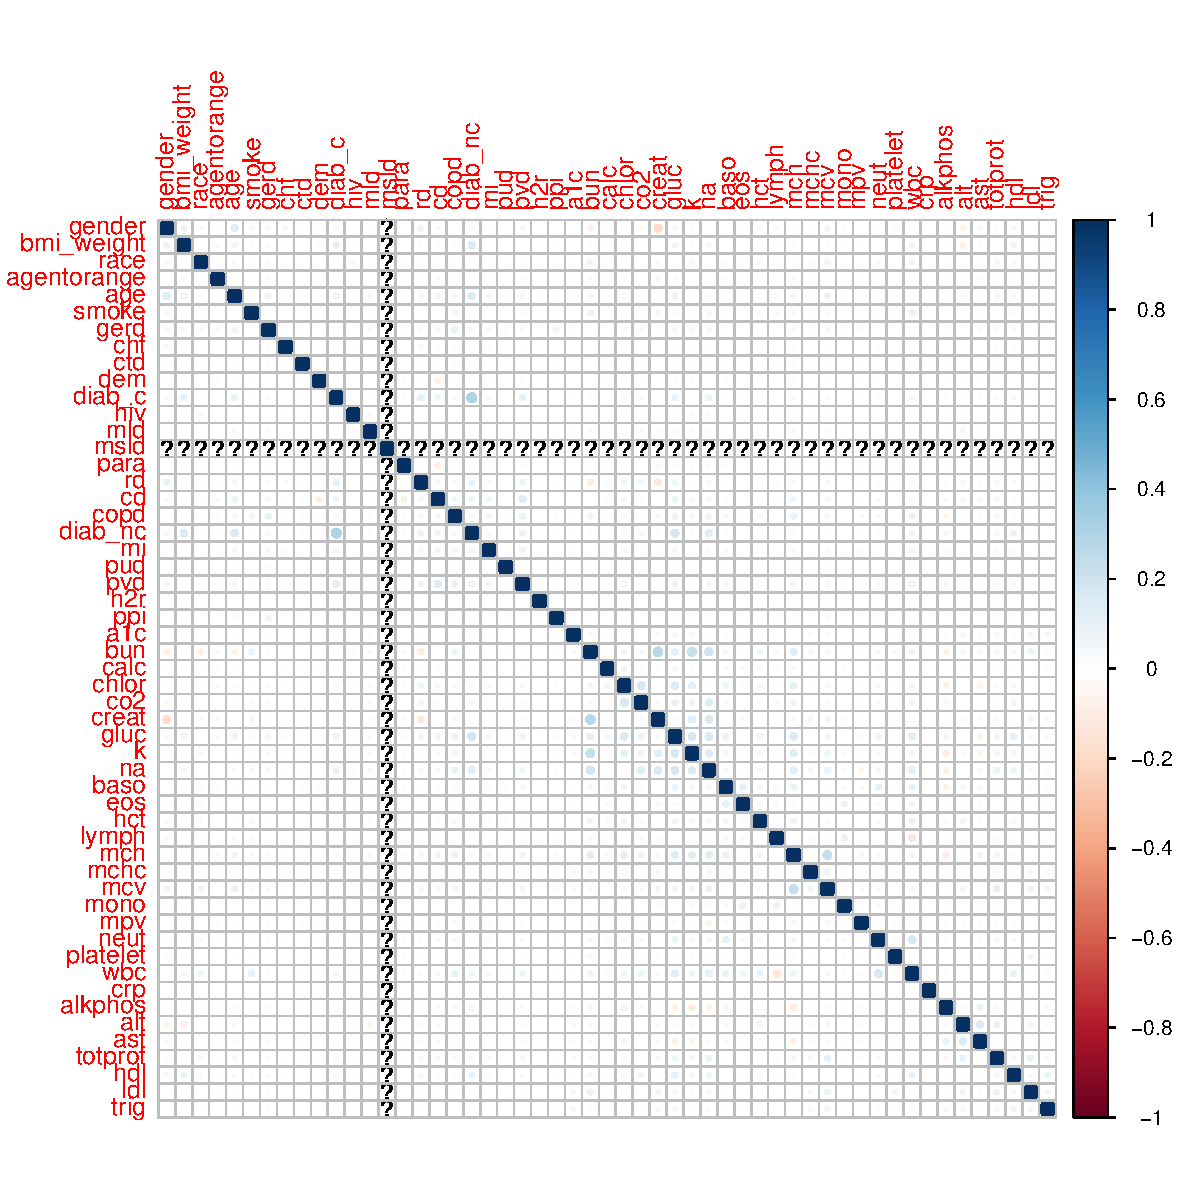
\includegraphics[width=0.96\textwidth]{figures/shap_new/shap_corr.pdf}
\caption{Correlation between group-level Shapley values. Largest absolute correlation in the following table. If two Shapley values
are highly correlated, that means the underlying variables contribute essentially in the same way to the prediction and are therefore redundant.}
\end{figure}

\clearpage
\begin{table}[h]
\centering
\begin{tabular}{llr}
\toprule
\multicolumn{2}{l}{Feature pair} & SHAP correlation \\
\midrule
diab\_c & diab\_nc & 0.31 \\ 
bun & creat & 0.28 \\ 
bun & k & 0.24 \\ 
mch & mcv & 0.23 \\ 
bun & na & 0.19 \\ \addlinespace
gender & creat & -0.18 \\ 
diab\_nc & gluc & 0.18 \\ 
chlor & co2 & 0.17 \\ 
gluc & k & 0.17 \\ 
neut & wbc & 0.17 \\ \addlinespace
gluc & na & 0.17 \\ 
creat & na & 0.16 \\ 
age & diab\_nc & 0.16 \\ 
chlor & gluc & 0.15 \\ 
bmi\_weight & diab\_nc & 0.15 \\ \addlinespace
alt & ast & 0.15 \\ 
k & na & 0.14 \\ 
gluc & mch & 0.14 \\ 
gender & age & 0.14 \\ 
cd & pvd & 0.14 \\  
\bottomrule
\end{tabular}
\caption{Since the largest Shapley correaltion is fairly low, we can be reassured we do not have redundant variables.
Is the top one resulting from patients haveing diab\_nc first and then diab\_c later?}
\end{table}


\clearpage
\section*{Identity groups}

\begin{center}
\includegraphics[width=\textwidth]{figures/roc_age.pdf}
\end{center}

\begin{center}
\includegraphics[width=\textwidth]{figures/roc_Race.pdf}
\end{center}

\begin{center}
\includegraphics[width=\textwidth]{figures/roc_gender.pdf}
\end{center}



\clearpage
\newpage
\newpage
\newpage


\clearpage
\section*{Cancer stage}

\begin{table}[ht]
\centering
\begin{tabular}{lrr}
  \toprule
 Stage & Test. AUC & Nb. cases \\ 
  \midrule
Any & 0.773 [0.765,0.78] & 2810 \\ \addlinespace
  I & 0.795 [0.773,0.817] & 298 \\ 
  II & 0.798 [0.774,0.822] & 240 \\ 
  III & 0.772 [0.757,0.787] & 631 \\ 
  IV & 0.767 [0.755,0.778] & 1041 \\  \addlinespace
  I+ & 0.775 [0.767,0.783] & 2254 \\ 
  II+ & 0.772 [0.764,0.78] & 1956 \\ 
  III+ & 0.768 [0.759,0.777] & 1716 \\ 
  IV+ & 0.767 [0.755,0.778] & 1041 \\ 
   \bottomrule
\end{tabular}
\caption{Interestingly, it seems slightly harder to predict late stages?}
\end{table}

\begin{figure}[h]
\centering
\includegraphics[width=1.0\textwidth]{figures/risk_stage.pdf}
\end{figure}



%
%\clearpage
%\section*{Lab variables interpretation}
%
%\begin{itemize}
%\item I started to look at ways we could interpret the effect of the lab variables on the predictions
%\item I focused on \texttt{mch} for now to develop the approach
%\item During this, I noticed that the labels for maxdiff and mindiff were flipped ... This doesn't change anything about performance though.
%\item same thing for min and max ...
%%\item Some important fact is that when tv is 0, maxdiff (mindiff) is negative or mindiff (maxdiff) is positive, that means there are just a few observations
%%since random variations trhough any signal should occur. This means any switch around these points indicate that the model is mostly learning 
%%that the patient had few observations for that variable ...
%%\item Maybe we should require, say, 5 observations for tv, mindiff, maxdiff? Should we include meandiff to get the overall trend?
%\end{itemize}
%
%\begin{figure}[h]
%\centering
%\includegraphics[width=1.0\textwidth]{figures/shap_new/shap_lab_mch.pdf}
%\caption{SHAP values for a sample with overrepresentation of cases ranked according to \texttt{mean|SHAP|} from top 
%to bottom.}
%\end{figure}
%
%\begin{figure}[h]
%\centering
%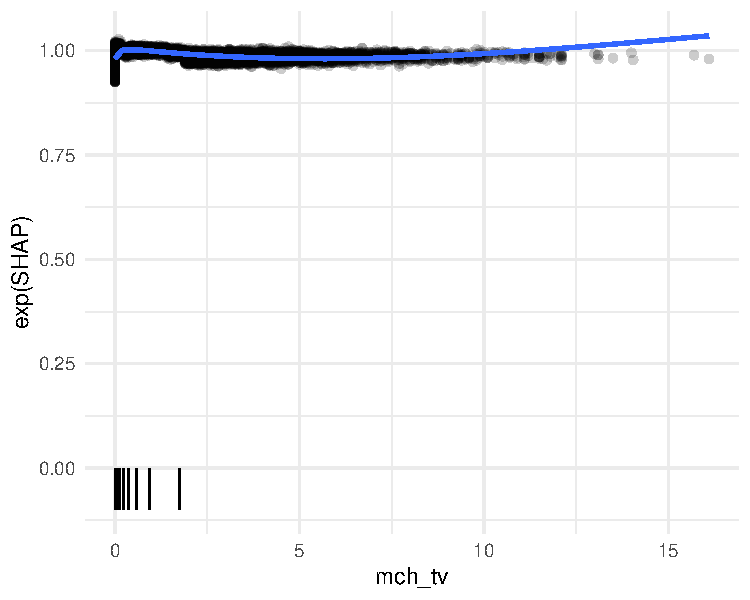
\includegraphics[width=0.49\textwidth]{figures/shap_new/mch_tv.pdf}
%\includegraphics[width=0.49\textwidth]{figures/shap_new/mch_maxdiff.pdf}
%\includegraphics[width=0.49\textwidth]{figures/shap_new/mch_mindiff.pdf}
%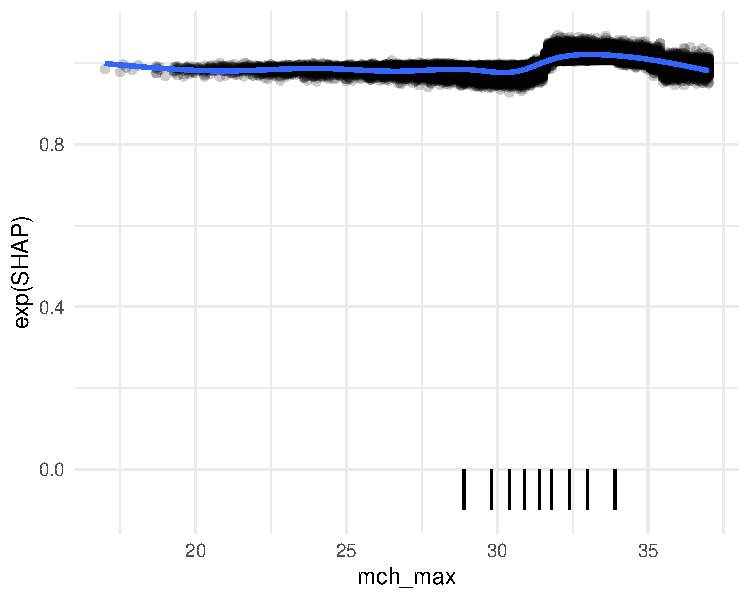
\includegraphics[width=0.49\textwidth]{figures/shap_new/mch_max.pdf}
%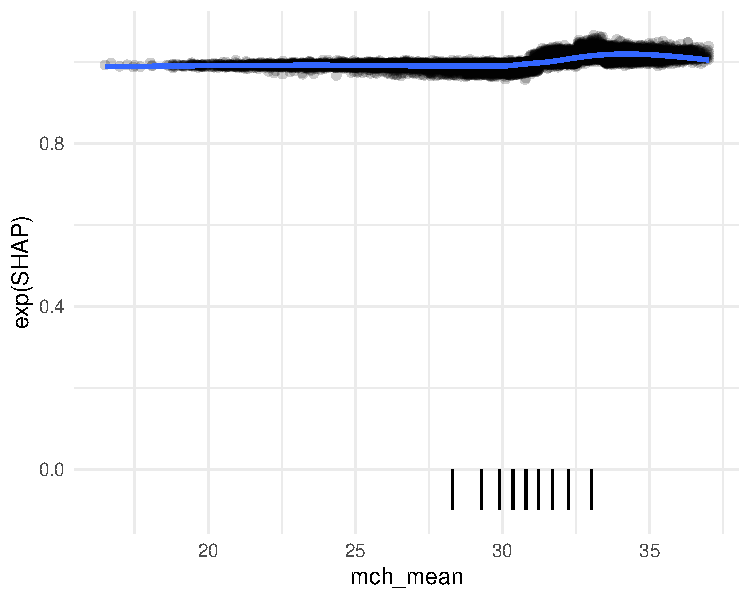
\includegraphics[width=0.49\textwidth]{figures/shap_new/mch_mean.pdf}
%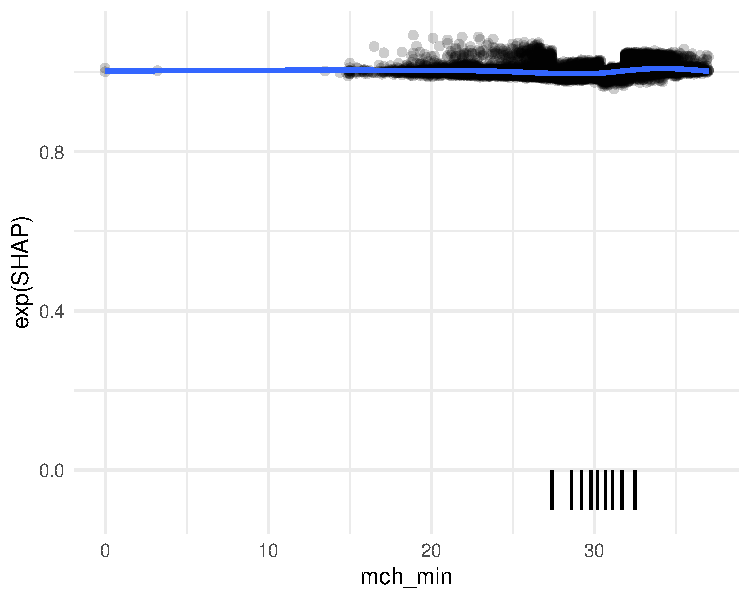
\includegraphics[width=0.49\textwidth]{figures/shap_new/mch_min.pdf}
%\caption{Very negative mindiff(maxdiff) means there is at least one large drop. 
%Very positive maxdiff (mindiff) means at least one large positive jump.
%Small max (min) means always small. Large min (max) means always large.}
%\end{figure}
%
%\begin{figure}[h]
%\centering
%\includegraphics[width=1.0\textwidth]{figures/lab/mch.pdf}
%\caption{Sample of trajectories of mch lab results. Left: stratified by their aggregated SHAP values. Right: straified by case/control status. 
%It is not obvious why some time series have low/high SHAP values just by looking at this, but we at least see that drop towards the end seem
%to be well separated.}
%\end{figure}
%
%\begin{figure}[h]
%\centering
%\includegraphics[width=1.0\textwidth]{figures/n_mch.png}
%\caption{It seems that patients with very few lab results indeed have higher predicted risk due to \texttt{mch}.}
%\end{figure}




\clearpage

\section*{Years prior}



\begin{figure}[h]
\centering
\includegraphics[width=1.0\textwidth]{figures/roc_window_2.pdf}
\caption{In this experiment, all three test set utilizes the same amount of data (2 years), 
but we predict farther in the future (1yr, 2yrs or 3yrs). As expected, we do worse and worse
as we predict further in time, but only by a small margin. This seem to indicate our predictions are 
somewhat valid beyond the 1yr window we used.}
\end{figure}



\begin{figure}[h]
\centering
\includegraphics[width=1.0\textwidth]{figures/roc_window_x-1.pdf}
\caption{In this experiment, we decrease the amount of data (from 4yrs to 1yr) in the test set, 
but keep the prediction horizon to 1yr. Performance only seem to decrease when dropping from 2 to 1 year of data.}
\end{figure}



\clearpage
\section*{EAC v EGJAC}

\begin{itemize}
	\item This is now looking a lot better now
	\item Almost no difference in features
	\item No difference in missing values (though there still is between Cases and Controls)
	\item 
\end{itemize}

\begin{table}[ht]
\centering
\begin{tabular}{lccc}
  \toprule
  & \multicolumn{3}{c}{Training on ...} \\ \cmidrule(l){2-4}
Testing on ... & ANY & EAC & EGJAC \\ 
  \midrule
ANY & 0.774 [0.766,0.781] & 0.768 [0.761,0.776] & 0.745 [0.737,0.752] \\ 
  EAC & 0.778 [0.770,0.786] & 0.775 [0.767,0.784] & 0.747 [0.738,0.755] \\ 
  EGJAC & 0.761 [0.746,0.776] & 0.747 [0.732,0.763] & 0.738 [0.723,0.754] \\ 
   \bottomrule
\end{tabular}
\caption{It seems that testing on EAC yields the best result all the time interestingly.}
\end{table}


\begin{figure}[h]
\centering
\includegraphics[width=0.8\textwidth]{figures/eac_v_egjac/risk_distribution_ANY.pdf}
\includegraphics[width=0.8\textwidth]{figures/eac_v_egjac/risk_distribution_EAC.pdf}
\includegraphics[width=0.8\textwidth]{figures/eac_v_egjac/risk_distribution_EGJAC.pdf}
\caption{Predicted risk don't go as large as before, there are essentially none above 1,000/100,000. For EGJAC, there is almost none beyond 150/100,000.
For EGJAC, the spread is smaller, which indicates less certainty by the model, and this transpires in the lower AUC. For ANY and EAC, the risk
distribution for EAC and EGJAC seem very similar. We also note two modes within the cases: risk between 1 and 10 and between 50 and 500.}
\end{figure}


\begin{figure}[h]
\centering
\includegraphics[width=1.0\textwidth]{figures/eac_v_egjac/risk_scatter.pdf}
\caption{Scatter plots of (log) predicted risk by all three models stratified by 
case/control status (none, EAC, EGJAC). We have almost perfect correlation between ANY and EAC risks within Controls and EGJAC,
while the correlation drops for EAC, indicating that the EAC-only model learns something somewhat different. There is better agreement
on controls and EGJAC between EAC and EGJAC models than between ANY and EGJAC models.
Within EAC, the highest correlation is
between ANY and EAC; within EGJAC, the highest correlation is also between ANY and EGJAC, which seems to indicate our EGJAC is doing worse.}
\end{figure}

\begin{figure}[h]
\centering
\includegraphics[width=1.0\textwidth]{figures/eac_v_egjac/shap_groups_cancertype.pdf}
\caption{SHAP variable importance wihtin all three models. Notably, we see large differences
\texttt{age}, \texttt{race}, \texttt{gender}, \texttt{gerd}, \texttt{bmi/weight}, \texttt{smoke}, and a few others.}
\end{figure}


%\begin{figure}[h]
%\centering
%\includegraphics[width=1.0\textwidth]{figures/eac_v_egjac/vs_shap_groups.pdf}
%\caption{SHAP variable importance for a model differentiating EAC from EGJAC. We
%again find \texttt{race}, \texttt{gluc}, \texttt{ppi}, \texttt{mpv} and \texttt{age} at the top}
%\end{figure}




\begin{table}[ht]
\centering
\begin{tabular}{lrrrr}
\hline
& Mean (control) & Mean (EAC) & Mean (EGJAC) & pvalue.adj \\
\hline
black & 0.169 & 0.041 & 0.089 & 0.001 \\ 
  gerd & 0.232 & 0.357 & 0.269 & 0.005 \\ 
  baso\_max & 1.017 & 0.328 & 1.791 & 0.033 \\ 
\hline
\end{tabular}
\caption{Features with different means between EAC and EGJAC (at 5\% level, BH). It appears that race and GERD are less important for EGJAC. 
We also find that baso could be different between the two.}
\end{table}



\clearpage

\begin{table}[ht]
\centering
\begin{tabular}{lrrrr}
\toprule
& Prop. Control & Prop. EAC & Prop. EGJAC & P-value (adj.) \\ 
\midrule
\\
\bottomrule
\end{tabular}
\caption{Features with different proportions of non-NAs between EAC and EGJAC (at 5\% level, BH).
There are None!}
\end{table}


\begin{figure}[h]
\centering
\includegraphics[width=0.8\textwidth]{figures/eac_v_egjac/vs_propNA.pdf}
\caption{No issues with missing proportions!}
\end{figure}



\subsubsection*{EAC Thrashold}

\begin{minipage}{0.5\textwidth}\small
\begin{tabular}{rccc}
\toprule
\textbf{Threshold} & \textbf{TPR} 
& \textbf{PPV} & \textbf{Det. prev.} \\
\midrule

      5 & 99.65 & 0.13 & 82.06 \\ 
     10 & 99.05 & 0.14 & 75.94 \\ 
     15 & 98.41 & 0.15 & 72.68 \\ 
     20 & 97.60 & 0.15 & 69.72 \\ 
     25 & 96.65 & 0.16 & 66.87 \\ \addlinespace
     30 & 95.52 & 0.16 & 64.09 \\ 
     35 & 94.17 & 0.17 & 61.37 \\ 
     40 & 92.69 & 0.17 & 58.70 \\ 
     45 & 91.35 & 0.18 & 56.08 \\ 
     50 & 89.62 & 0.18 & 53.50 \\  \addlinespace
     55 & 87.96 & 0.19 & 51.01 \\ 
     60 & 86.30 & 0.20 & 48.54 \\ 
     65 & 84.36 & 0.20 & 46.15 \\ 
     70 & 82.94 & 0.21 & 43.83 \\ 
     75 & 80.86 & 0.21 & 41.57 \\  \addlinespace
     80 & 79.24 & 0.22 & 39.37 \\ 
     85 & 77.01 & 0.23 & 37.23 \\ 
     90 & 74.89 & 0.23 & 35.18 \\ 
     95 & 72.21 & 0.24 & 33.19 \\ 
    100 & 69.95 & 0.25 & 31.29 \\  \addlinespace
    105 & 67.55 & 0.25 & 29.46 \\ 
    110 & 65.22 & 0.26 & 27.73 \\ 
    115 & 62.99 & 0.27 & 26.06 \\ 
    120 & 60.49 & 0.27 & 24.50 \\ 
    125 & 58.40 & 0.28 & 23.02 \\  \addlinespace
    130 & 56.00 & 0.29 & 21.64 \\ 
    135 & 53.67 & 0.29 & 20.31 \\ 
    140 & 51.69 & 0.30 & 19.07 \\ 
    145 & 49.68 & 0.31 & 17.91 \\ 
    150 & 47.88 & 0.31 & 16.81 \\  \addlinespace
    155 & 45.87 & 0.32 & 15.80 \\ 
    160 & 44.53 & 0.33 & 14.83 \\ 
    165 & 42.16 & 0.33 & 13.94 \\ 
    170 & 40.22 & 0.34 & 13.10 \\ 
    175 & 38.95 & 0.35 & 12.33 \\  \addlinespace
    180 & 37.75 & 0.36 & 11.60 \\ 
    185 & 36.48 & 0.37 & 10.93 \\ 
    190 & 35.45 & 0.38 & 10.30 \\ 
    195 & 34.25 & 0.39 & 9.70 \\ 
    200 & 32.27 & 0.39 & 9.14 \\ 

\bottomrule
\end{tabular}

\end{minipage} \hfill
\begin{minipage}{0.5\textwidth}\small
\begin{tabular}{rccc}
\toprule
\textbf{Threshold} & \textbf{TPR} 
& \textbf{PPV} & \textbf{Det. prev.} \\
\midrule 
    210 & 29.94 & 0.41 & 8.12 \\ 
    220 & 27.72 & 0.42 & 7.24 \\ 
    230 & 25.53 & 0.44 & 6.47 \\ 
    240 & 23.52 & 0.45 & 5.79 \\ 
    250 & 21.15 & 0.45 & 5.18 \\  \addlinespace
    260 & 19.56 & 0.46 & 4.65 \\ 
    270 & 18.26 & 0.48 & 4.18 \\ 
    280 & 17.20 & 0.50 & 3.76 \\ 
    290 & 15.75 & 0.51 & 3.39 \\ 
    300 & 14.30 & 0.52 & 3.06 \\  \addlinespace
    325 & 12.04 & 0.56 & 2.38 \\ 
    350 & 9.96 & 0.59 & 1.87 \\ 
    375 & 8.02 & 0.60 & 1.47 \\ 
    400 & 6.64 & 0.63 & 1.17 \\ 
    425 & 5.58 & 0.66 & 0.93 \\  \addlinespace
    450 & 4.27 & 0.63 & 0.75 \\ 
    475 & 3.71 & 0.68 & 0.60 \\ 
    500 & 2.75 & 0.63 & 0.49 \\ 
    600 & 1.20 & 0.61 & 0.22 \\ 
    700 & 0.85 & 0.91 & 0.10 \\  \addlinespace
    800 & 0.42 & 0.91 & 0.05 \\ 
    900 & 0.18 & 0.70 & 0.03 \\ 
   1000 & 0.11 & 0.73 & 0.02 \\ 
   1100 & 0.04 & 0.42 & 0.01 \\ 
   1200 & 0.04 & 0.61 & 0.01 \\  \addlinespace
   1300 & 0.00 & 0.00 & 0.00 \\ 
   1400 & 0.00 & 0.00 & 0.00 \\ 
   1500 & 0.00 & 0.00 & 0.00 \\ 
   1600 & 0.00 & 0.00 & 0.00 \\ 
   1700 & 0.00 & 0.00 & 0.00 \\  \addlinespace
   1800 & 0.00 & 0.00 & 0.00 \\ 
   1900 & 0.00 & 0.00 & 0.00 \\ 
   2000 & 0.00 & 0.00 & 0.00 \\ 
   3000 & 0.00 & 0.00 & 0.00 \\ 
   4000 & 0.00 & 0.00 & 0.00 \\  \addlinespace
   5000 & 0.00 & 0.00 & 0.00 \\ 
   6000 & 0.00 & 0.00 & 0.00 \\ 
   7000 & 0.00 & 0.00 & 0.00 \\ 
   8000 & 0.00 & 0.00 & 0.00 \\ 
  10000 & 0.00 & 0.00 & 0.00 \\ 
\bottomrule
\end{tabular}

\end{minipage}





\subsubsection*{EGJAC Thrashold}

\begin{minipage}{0.5\textwidth}\small
\begin{tabular}{rccc}
\toprule
\textbf{Threshold} & \textbf{TPR} 
& \textbf{PPV} & \textbf{Det. prev.} \\
\midrule

      5 & 99.39 & 0.13 & 80.54 \\ 
     10 & 99.04 & 0.14 & 77.35 \\ 
     15 & 97.83 & 0.15 & 72.34 \\ 
     20 & 95.26 & 0.16 & 64.80 \\ 
     25 & 89.02 & 0.18 & 55.36 \\  \addlinespace
     30 & 80.54 & 0.20 & 44.87 \\ 
     35 & 69.53 & 0.22 & 34.55 \\ 
     40 & 58.13 & 0.25 & 25.80 \\ 
     45 & 48.11 & 0.27 & 19.27 \\ 
     50 & 38.28 & 0.29 & 14.62 \\  \addlinespace
     55 & 31.68 & 0.31 & 11.26 \\ 
     60 & 26.05 & 0.33 & 8.76 \\ 
     65 & 21.70 & 0.35 & 6.81 \\ 
     70 & 17.64 & 0.37 & 5.26 \\ 
     75 & 13.86 & 0.38 & 4.02 \\  \addlinespace
     80 & 10.91 & 0.39 & 3.02 \\ 
     85 & 7.95 & 0.38 & 2.26 \\ 
     90 & 6.41 & 0.42 & 1.66 \\ 
     95 & 4.78 & 0.43 & 1.20 \\ 
    100 & 3.53 & 0.44 & 0.87 \\  \addlinespace
    105 & 2.46 & 0.43 & 0.62 \\ 
    110 & 1.96 & 0.49 & 0.44 \\ 
    115 & 1.43 & 0.51 & 0.31 \\ 
    120 & 1.00 & 0.50 & 0.22 \\ 
    125 & 0.86 & 0.60 & 0.16 \\  \addlinespace
    130 & 0.57 & 0.56 & 0.11 \\ 
    135 & 0.46 & 0.65 & 0.08 \\ 
    140 & 0.36 & 0.70 & 0.06 \\ 
    145 & 0.21 & 0.62 & 0.04 \\ 
    150 & 0.14 & 0.56 & 0.03 \\  \addlinespace
    155 & 0.11 & 0.60 & 0.02 \\ 
    160 & 0.11 & 0.87 & 0.01 \\ 
    165 & 0.07 & 0.81 & 0.01 \\ 
    170 & 0.04 & 0.62 & 0.01 \\ 
    175 & 0.04 & 1.03 & 0.00 \\  \addlinespace
    180 & 0.04 & 1.59 & 0.00 \\ 
    185 & 0.04 & 2.50 & 0.00 \\ 
    190 & 0.00 & 0.00 & 0.00 \\ 
    195 & 0.00 & 0.00 & 0.00 \\ 
    200 & 0.00 & 0.00 & 0.00 \\  

\bottomrule
\end{tabular}

\end{minipage} \hfill
\begin{minipage}{0.5\textwidth}\small
\begin{tabular}{rccc}
\toprule
\textbf{Threshold} & \textbf{TPR} 
& \textbf{PPV} & \textbf{Det. prev.} \\
\midrule 
    210 & 0.00 & 0.00 & 0.00 \\ 
    220 & 0.00 & 0.00 & 0.00 \\ 
    230 & 0.00 &  & 0.00 \\ 
    240 & 0.00 &  & 0.00 \\ 
    250 & 0.00 &  & 0.00 \\  \addlinespace
    260 & 0.00 &  & 0.00 \\ 
    270 & 0.00 &  & 0.00 \\ 
    280 & 0.00 &  & 0.00 \\ 
    290 & 0.00 &  & 0.00 \\ 
    300 & 0.00 &  & 0.00 \\  \addlinespace
    325 & 0.00 &  & 0.00 \\ 
    350 & 0.00 &  & 0.00 \\ 
    375 & 0.00 &  & 0.00 \\ 
    400 & 0.00 &  & 0.00 \\ 
    425 & 0.00 &  & 0.00 \\  \addlinespace
    450 & 0.00 &  & 0.00 \\ 
    475 & 0.00 &  & 0.00 \\ 
    500 & 0.00 &  & 0.00 \\ 
    600 & 0.00 &  & 0.00 \\ 
    700 & 0.00 &  & 0.00 \\  \addlinespace
    800 & 0.00 &  & 0.00 \\ 
    900 & 0.00 &  & 0.00 \\ 
   1000 & 0.00 &  & 0.00 \\ 
   1100 & 0.00 &  & 0.00 \\ 
   1200 & 0.00 &  & 0.00 \\  \addlinespace
   1300 & 0.00 &  & 0.00 \\ 
   1400 & 0.00 &  & 0.00 \\ 
   1500 & 0.00 &  & 0.00 \\ 
   1600 & 0.00 &  & 0.00 \\ 
   1700 & 0.00 &  & 0.00 \\  \addlinespace
   1800 & 0.00 &  & 0.00 \\ 
   1900 & 0.00 &  & 0.00 \\ 
   2000 & 0.00 &  & 0.00 \\ 
   3000 & 0.00 &  & 0.00 \\ 
   4000 & 0.00 &  & 0.00 \\  \addlinespace
   5000 & 0.00 &  & 0.00 \\ 
   6000 & 0.00 &  & 0.00 \\ 
   7000 & 0.00 &  & 0.00 \\ 
   8000 & 0.00 &  & 0.00 \\ 
  10000 & 0.00 &  & 0.00 \\ 
\bottomrule
\end{tabular}

\end{minipage}



\subsubsection*{Data comparison}

\begin{table}[ht]
\centering
\begin{tabular}{llrrrrrrr}
  \toprule
variable & cancertype & old & new & diff & Is diff. (\%) & NA-NA (\%) & Obs-NA(\%)& NA-Obs.(\%) \\ 
  \midrule
  alkphos & EAC & 86.02 & 86.14 & 0.00 & 0.43 & 42.04 & 0.07 & 10.94 \\ 
   & EGJAC & 85.55 & 85.83 & 0.01 & 0.47 & 44.41 & 0.06 & 11.99 \\ 
   & All & 85.89 & 86.06 & 0.00 & 0.44 & 42.70 & 0.06 & 11.23 \\ \addlinespace
  alt & EAC & 32.52 & 32.56 & 0.00 & 0.52 & 36.34 & 0.08 & 11.59 \\ 
   & EGJAC & 31.86 & 31.52 & -0.01 & 0.36 & 38.57 & 0.08 & 12.91 \\ 
   & All & 32.34 & 32.28 & -0.00 & 0.48 & 36.96 & 0.08 & 11.96 \\  \addlinespace
  ast & EAC & 30.00 & 30.00 & -0.01 & 0.36 & 37.63 & 0.08 & 11.36 \\ 
   & EGJAC & 29.56 & 29.54 & -0.00 & 0.39 & 40.38 & 0.07 & 12.67 \\ 
   & All & 29.88 & 29.88 & -0.01 & 0.37 & 38.39 & 0.08 & 11.73 \\  \addlinespace
  totprot & EAC & 7.01 & 7.01 & -0.00 & 0.62 & 52.92 & 0.00 & 0.00 \\ 
   & EGJAC & 7.03 & 7.03 & 0.00 & 0.53 & 55.71 & 0.00 & 0.00 \\ 
   & All & 7.02 & 7.02 & 0.00 & 0.59 & 53.70 & 0.00 & 0.00 \\  \addlinespace
  baso & EAC & 0.22 & 0.22 & 0.00 & 0.00 & 50.35 & 0.00 & 0.00 \\ 
   & EGJAC & 0.47 & 0.47 & 0.00 & 0.00 & 49.07 & 0.00 & 0.00 \\ 
   & All & 0.29 & 0.29 & 0.00 & 0.00 & 49.99 & 0.00 & 0.00 \\  \addlinespace
  eos & EAC & 0.85 & 0.85 & 0.00 & 0.00 & 47.63 & 0.00 & 0.00 \\ 
   & EGJAC & 1.30 & 1.30 & 0.00 & 0.00 & 47.80 & 0.00 & 0.00 \\ 
   & All & 0.97 & 0.97 & 0.00 & 0.00 & 47.68 & 0.00 & 0.00 \\  \addlinespace
  hct & EAC & 39.84 & 39.84 & -0.00 & 1.96 & 20.70 & 0.21 & 0.36 \\ 
   & EGJAC & 40.80 & 39.22 & 0.03 & 1.88 & 19.74 & 1.46 & 78.37 \\ 
   & All & 39.84 & 39.67 & 0.00 & 1.96 & 20.43 & 0.56 & 22.08 \\  \addlinespace
  hgb & EAC & 13.54 & 13.54 & 0.00 & 0.00 & 20.65 & 0.00 & 0.00 \\ 
   & EGJAC & 13.30 & 13.30 & 0.00 & 0.00 & 22.33 & 0.00 & 0.00 \\ 
   & All & 13.47 & 13.47 & 0.00 & 0.00 & 21.12 & 0.00 & 0.00 \\  \addlinespace
  lymph & EAC & 3.45 & 3.43 & -0.00 & 5.99 & 46.95 & 0.17 & 0.28 \\ 
   & EGJAC & 2.52 & 3.76 & -0.12 & 0.60 & 45.68 & 1.06 & 52.98 \\ 
   & All & 3.44 & 3.52 & -0.01 & 5.98 & 46.60 & 0.41 & 14.95 \\  \addlinespace
  mch & EAC & 30.62 & 30.63 & 0.00 & 2.83 & 20.17 & 0.20 & 0.39 \\ 
   & EGJAC & 31.06 & 30.45 & -0.00 & 1.14 & 19.94 & 1.45 & 78.19 \\ 
   & All & 30.63 & 30.58 & 0.00 & 2.83 & 20.10 & 0.55 & 22.05 \\  \addlinespace
   \bottomrule
\end{tabular}
\end{table}



\begin{table}[ht]
\centering
\begin{tabular}{llrrrrrrr}
  \toprule
variable & cancertype & old & new & diff & Is diff. (\%) & NA-NA (\%) & Obs-NA(\%)& NA-Obs.(\%) \\ 
  \midrule
  mchc & EAC & 33.65 & 33.65 & 0.00 & 0.00 & 22.65 & 0.00 & 0.00 \\ 
   & EGJAC & 33.51 & 33.51 & 0.00 & 0.00 & 24.23 & 0.00 & 0.00 \\ 
   & All & 33.61 & 33.61 & 0.00 & 0.00 & 23.09 & 0.00 & 0.00 \\  \addlinespace
  mcv & EAC & 90.03 & 90.03 & 0.00 & 0.00 & 23.02 & 0.00 & 0.00 \\ 
   & EGJAC & 89.68 & 89.68 & 0.00 & 0.00 & 24.24 & 0.00 & 0.00 \\ 
   & All & 89.94 & 89.94 & 0.00 & 0.00 & 23.36 & 0.00 & 0.00 \\  \addlinespace
  mono & EAC & 1.38 & 1.38 & 0.00 & 0.00 & 50.90 & 0.00 & 0.00 \\ 
   & EGJAC & 1.44 & 1.44 & 0.00 & 0.00 & 51.51 & 0.00 & 0.00 \\ 
   & All & 1.40 & 1.40 & 0.00 & 0.00 & 51.07 & 0.00 & 0.00 \\  \addlinespace
  mpv & EAC & 9.05 & 9.05 & 0.00 & 0.00 & 38.72 & 0.00 & 0.00 \\ 
   & EGJAC & 9.19 & 9.19 & 0.00 & 0.00 & 40.84 & 0.00 & 0.00 \\ 
   & All & 9.09 & 9.09 & 0.00 & 0.00 & 39.31 & 0.00 & 0.00 \\  \addlinespace
  neut & EAC & 8.54 & 8.48 & -0.06 & 4.65 & 52.02 & 0.00 & 0.00 \\ 
   & EGJAC & 8.55 & 8.60 & 0.06 & 4.94 & 53.24 & 0.00 & 0.00 \\ 
   & All & 8.54 & 8.52 & -0.02 & 4.73 & 52.36 & 0.00 & 0.00 \\  \addlinespace
  platelet & EAC & 236.13 & 236.13 & 0.00 & 0.00 & 19.80 & 0.00 & 0.00 \\ 
   & EGJAC & 235.36 & 235.36 & 0.00 & 0.00 & 21.08 & 0.00 & 0.00 \\ 
   & All & 235.92 & 235.92 & 0.00 & 0.00 & 20.16 & 0.00 & 0.00 \\  \addlinespace
  rbc & EAC & 4.44 & 4.44 & 0.00 & 0.00 & 19.34 & 0.00 & 0.00 \\ 
   & EGJAC & 4.38 & 4.38 & 0.00 & 0.00 & 20.62 & 0.00 & 0.00 \\ 
   & All & 4.42 & 4.42 & 0.00 & 0.00 & 19.69 & 0.00 & 0.00 \\  \addlinespace
  rdw & EAC & 15.04 & 15.04 & 0.00 & 0.00 & 21.32 & 0.00 & 0.00 \\ 
   & EGJAC & 14.99 & 14.99 & 0.00 & 0.00 & 23.05 & 0.00 & 0.00 \\ 
   & All & 15.03 & 15.03 & 0.00 & 0.00 & 21.80 & 0.00 & 0.00 \\  \addlinespace
  wbc & EAC & 8.23 & 8.23 & 0.00 & 0.00 & 19.75 & 0.00 & 0.00 \\ 
   & EGJAC & 8.13 & 8.13 & 0.00 & 0.00 & 20.72 & 0.00 & 0.00 \\ 
   & All & 8.20 & 8.20 & 0.00 & 0.00 & 20.02 & 0.00 & 0.00 \\ 
   \bottomrule
\end{tabular}
\caption{Lots of values change for \texttt{hct}, \texttt{lymph}, \texttt{mch} and \texttt{neut}. 
Change of missing status frequent for \texttt{alkphos}, \texttt{alt}, and \texttt{ast}, but equally for both types;
very frequent for \texttt{hct}, \texttt{lymph}, \texttt{mch} only in EGJAC.}
\end{table}



\clearpage
\section*{Birth cohort effect}



\begin{figure}[h]
\centering
\includegraphics[width=\textwidth]{figures/birthyear/pdp_models.pdf}
\includegraphics[width=\textwidth]{figures/birthyear/shap_models.pdf}
\end{figure}



\begin{figure}[h]
\centering
\includegraphics[width=0.9\textwidth]{figures/birthyear/shap_num_age.pdf}
\includegraphics[width=0.9\textwidth]{figures/birthyear/shap_num_by.pdf}
\includegraphics[width=0.9\textwidth]{figures/birthyear/shap_num_age_by.pdf}
\end{figure}



\clearpage
\section*{Are we simply diagnosing cancer?}

Since WBC is the main lab result influencing predicted risk, we investigate its relationship to cancer stage.
\begin{itemize}
\item I decided to compare stage O/1 to II/III/IV
\item The main conclusion is that there is a gradient of effect following stage: 
the higher the stage, the higher the effect of WBC
\item I'm not sure this is the best approach to study this yet, but, so far, it doesn't seem too bad
\end{itemize}



\begin{figure}[h]
\centering
\includegraphics[width=\textwidth]{figures/diagnosing/wbc_mean.pdf}
\end{figure}
\begin{figure}[h]
\centering
\includegraphics[width=\textwidth]{figures/diagnosing/wbc_max.pdf}
\end{figure}
\begin{figure}[h]
\centering
\includegraphics[width=\textwidth]{figures/diagnosing/wbc_min.pdf}
\end{figure}




%\clearpage
%
%
%\section*{***Old stuff to update from here***}
%\section*{Feature selection}
%
%
%\textbf{Correlation}:
%
%%\begin{figure}[h]
%%\centering
%%\includegraphics[width=\textwidth]{figures/lab_corr.pdf}
%%\end{figure}
%
%\begin{table}[h]
%\centering
%\begin{tabular}{rllr}
%  \hline
% & var1 & var2 & correlation \\ 
%  \hline
%  2 & mchc & mch & 0.569 \\ 
%  3 & chlor & na & 0.578 \\ 
%  6 & creat & bun & 0.617 \\ 
%  8 & gluc & A1c & 0.707 \\ 
%  10 & mcv & mch & 0.742 \\ 
%  11 & alt & ast & 0.782 \\ 
%  13 & hgb & rbc & 0.857 \\ 
%  15 & chol & ldl & 0.875 \\ 
%  18 & rbc & hct & 0.884 \\ 
%  20 & hgb & hct & 0.976 \\ 
%   \hline
%\end{tabular}
%\caption{HGB and HCT are indeed very highly correlated}
%\end{table}
%
%\clearpage
%\textbf{On chol/ldl/hdl}:
%Missingness patterns does not help
%\begin{table}[h]
%\centering
%\begin{tabular}{lrrrrrrrr}
%\toprule
%Pattern (chol,hdl,ldl) & 000 & 001 & 010 & 011 & 100 & 101 & 110 & 111 \\
%\midrule
%Prop (\%) & 59.5 & 0.7 & 0.5 & 0.6 & 0.2 & 0.0 & 0.2 & 38.3\\
%\bottomrule
%\end{tabular}
%\end{table}
%
%\textbf{Using performance}:
%\begin{itemize}
%\item Drop various features:
%\begin{itemize}
%	\item (colonoscopy, fobt)
%	\item two of (hct, hgb, rct)
%	\item one or two of (chol, ldl, hdl)
%\end{itemize}
%\item Refit with 1M controls \& evaluate
%\item Proposed is dropping (colonoscopy, fobt, hbg, rct, chol)
%\item Conclusions:
%\begin{itemize}
%	\item Not much difference
%	\item Probably best to avoid dropping hct
%\end{itemize}
%\end{itemize}
%
%
%\begin{table}[ht]
%\centering
%\begin{tabular}{lrr}
%\toprule
%Drop & Valid. AUC & Test AUC \\
%\midrule
%None & 0.832 & 0.827 \\ \addlinespace
%Colonoscopy, fobt & 0.830 & 0.826 \\ \addlinespace
%rct, hgb & 0.831 & 0.826 \\
%rbc, hct & 0.824 & 0.821 \\
%hct, hgb & 0.824 & 0.826 \\ \addlinespace
%chol & 0.834 & 0.831 \\
%ldl & 0.831 & 0.829 \\
%hdl & 0.832 & 0.825 \\
%hdl, ldl & 0.831 & 0.830 \\ \addlinespace
%(proposed) & 0.827 & 0.827 \\
%\bottomrule
%\end{tabular}
%\end{table}




\end{document}
